\section{Współczynnik wydajności funkcji}\label{chapter:results_wwf}

\begin{figure}[h]
    \centering
    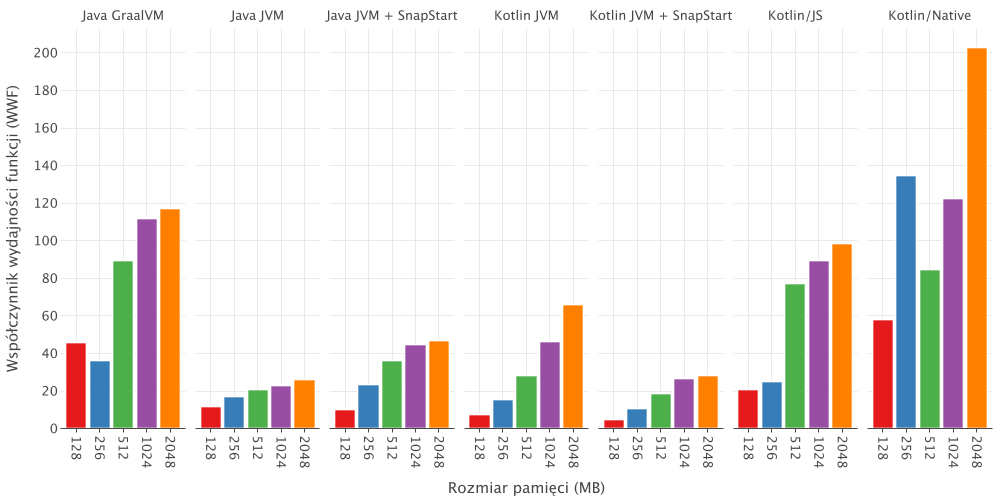
\includegraphics[width=0.95\textwidth]{charts/results/wwf.png}
    \caption{Współczynnik wydajności funkcji w zależności od rozmiaru pamięci [źródło: opracowanie własne]}
    \label{fig:avg_wwf}
\end{figure}

Kolejnym badanym kryterium jest współczynnik wydajności funkcji (WWF), opisany w Rozdziale \ref{chapter:cel_i_metodologia_badan}.
Pozwala on na jednoczesną analizę zarówno ciepłych, jak i zimnych startów, a wyższe wartości WWF oznaczają wyższą wydajność funkcji.
Wartości WWF zostały obliczone na bazie średnich czasów wykonania podczas zimnych i ciepłych startów.
W ramach obliczeń przyjęto wagi: 0,95 dla ciepłych startów oraz 0,05 dla zimnych startów.
Wyniki dla poszczególnych metod i rozmiarów pamięci zostały przedstawione na Rysunku \ref{fig:avg_wwf}.

Dla funkcji Java opartej o JVM, wartość współczynnika rośnie wraz z wzrostem pamięci.
Podobny trend występuje dla funkcji Kotlin JVM, gdzie jednak wzrost ten jest bardziej dynamiczny.
Dla małych rozmiarów pamięci funkcje Kotlin charakteryzują się mniejszą wydajnością, jednak zmienia się to dla wyższych wartości pamięci (od 512 MB wzyż).
Skuteczność użycia usługi SnapStart zależy od użytego języka programowania.
W przypadku Javy, wydajność poprawiła się dla wszystkich rozmiarów pamięci oprócz 128 MB. 
Dla Kotlina wydajność pogorszyła się (w porównaniu z funkcjami Kotlin JVM) dla wszystkich rozmiarów pamięci, gdzie wraz z zwiększaniem wielkości pamięci różnica pogłębia się.

Znaczną poprawę wydajności dla wszystkich rozmiarów pamięci zauważono w funkcjach Java GraalVM, Kotlin/JS oraz Kotlin/Native.
W przypadku dwóch pierwszych widoczny jest znaczny wzrost wartości WWF dla rozmiarów pamięci niemniejszych niż 512 MB.
Dla tych rozmiarów pamięci obie te funkcje wykazują podobną wydajność, jednak z przewagą dla funkcji Java GraalVM.
Przewaga ta jest znacznie większa dla mniejszych pojemności pamięci (128 MB i 256 MB).
Najlepszą wartością współczynnika charakteryzuje się jednak użycie Kotlin/Native, gdzie współczynnik osiągnął najlepsze wartość dla wszystkich rozmiarów pamięci oprócz 512 MB.
Jednak dla pamięci 512 MB, wartość WWF jest około 4\% niższa dla Kotlin/Native niż Java GraalVM.
Warte zwrócenia uwagi są jednak badania przeprowadzone dla rozmiarów pamięci 256 MB i 2048 MB, gdzie Kotlin/Native osiągnął znacznie wyższe wartości WWF niż pozostałe funkcje.
W porównaniu z Java GraalVM, czyli drugą najbardziej skuteczną metodą, wartości są wyższe o około 275\% i 74\%.
